\documentclass[12pt,a4paper]{article}
\usepackage[utf8]{inputenc}
\usepackage{dsfont} 
\usepackage[polish]{babel}
\usepackage{amsmath}
\usepackage{graphicx}
\usepackage[top=1in, bottom=1.5in, left=1.25in, right=1.25in]{geometry}
\usepackage{tocloft}
\usepackage{subfig}
\usepackage{multirow}
\usepackage{multicol}
\graphicspath{{Imagens/}}
\usepackage{xcolor,colortbl}
\usepackage{float}

\newcommand \comment[1]{\textbf{\textcolor{red}{#1}}}

%\usepackage{float}
\usepackage{fancyhdr} % Required for custom headers
\usepackage{extramarks} % Required for headers and footers
\usepackage{indentfirst}
\usepackage{placeins}
\usepackage{scalefnt}
\usepackage{xcolor,listings}
\usepackage{textcomp}
\usepackage{color}
\usepackage{verbatim}
\usepackage{framed}
\usepackage{subcaption}
\usepackage[T1]{fontenc}
\definecolor{codegreen}{rgb}{0,0.6,0}
\definecolor{codegray}{rgb}{0.5,0.5,0.5}
\definecolor{codepurple}{HTML}{C42043}
\definecolor{backcolour}{HTML}{F2F2F2}
\definecolor{bookColor}{cmyk}{0,0,0,0.90}  
\color{bookColor}

\lstset{upquote=true}

\lstdefinestyle{mystyle}{
	backgroundcolor=\color{backcolour},   
	commentstyle=\color{codegreen},
	keywordstyle=\color{codepurple},
	numberstyle=\numberstyle,
	stringstyle=\color{codepurple},
	basicstyle=\footnotesize\ttfamily,
	breakatwhitespace=false,
	breaklines=true,
	captionpos=b,
	keepspaces=true,
	numbers=left,
	numbersep=10pt,
	showspaces=false,
	showstringspaces=false,
	showtabs=false,
}
\lstset{style=mystyle}

\newcommand\numberstyle[1]{%
	\footnotesize
	\color{codegray}%
	\ttfamily
	\ifnum#1<10 0\fi#1 |%
}

\definecolor{shadecolor}{HTML}{F2F2F2}

\newenvironment{sqltable}%
{\snugshade\verbatim}%
{\endverbatim\endsnugshade}

% Margins
\addtolength{\footskip}{0cm}
\addtolength{\textwidth}{1.4cm}
\addtolength{\oddsidemargin}{-.7cm}

\addtolength{\textheight}{1.6cm}
%\addtolength{\topmargin}{-2cm}

% paragrafo
\addtolength{\parskip}{.2cm}

% Set up the header and footer
\pagestyle{fancy}
\rhead{\hmwkAuthorName} % Top left header
\lhead{\hmwkTitle} % Top center header
\rhead{\firstxmark} % Top right header
\renewcommand{\headrulewidth}{1pt}
\renewcommand{\footrulewidth}{1pt}

    
\newcommand{\hmwkTitle}{Algorytmy Numeryczne: Zadanie 1}
\newcommand{\hmwkDueDate}{\today}
\newcommand{\hmwkClass}{Algorytmy Numeryczne}
\newcommand{\hmwkAuthorName}{Maria Koren}


\renewcommand{\cftsecleader}{\cftdotfill{\cftdotsep}}
\renewcommand{\cftsubsecleader}{\cftdotfill{\cftdotsep}}
\renewcommand{\cftsubsubsecleader}{\cftdotfill{\cftdotsep}}

% trabalho 
\begin{document}
% capa
\begin{titlepage}
    \vfill
	\begin{center}
	\hspace*{-1cm}
	\vspace*{0.5cm}
    
\includegraphics[scale=0.55]{images/loga.png}\\
	\textbf{Uniwersytet Gdański \\ [0.05cm]Wydział Matematyki, Fizyki i Informatyki \\ [0.05cm] Instytut Informatyki}

	\vspace{0.6cm}
	\vspace{4cm}
	{\huge \textbf{\hmwkTitle}}\vspace{8mm}
	
	{\large \textbf{\hmwkAuthorName}}\\[3cm]
	

	  \vfill
	\textbf{Gdańsk}
	
	\textbf{\hmwkDueDate}
	\end{center}
	
\end{titlepage}

\newpage
\tableofcontents{}
\newpage

\section{Wstęp}


W tym projekcie zostało obliczono znaczenie liczby $\pi$ za pomocą dwóch metod, oraz sprawdzowno pewne hipotezy odnośnie tych metod.

Pierwsza metoda polegała na obliczeniu obwodu $n$-kąta foremnego wpisanego w okrąg o promieniu 1. Dla dużych $n$ obwód wpisanego wielokąta jest bliski obwodowi okręgu, który wynosi $2\Pi$

Druga metoda - Metoda Monte Carlo. Wylosowano $n$ punktów na płaszczyźnie, obie współrzędne z przedziału $[0, 1]$. Dalej obliczono ile z wylosowanych punktów mają odległość od punktu $(0, 0)$ nie większą niż 1, liczbę takich punktów oznaczono jako $a$. Iloraz $4a/n$ stanowi przybliżenie liczby $\Pi$

\newpage

\section{Hipoteza 1: Zwiększając $n$ można uzyskać obwód dowolnie bliski liczbie $2\Pi$}

W celu sprawdzenia tej hipotezy obliczono obwody dla różnych $n$-kątów. Były wzięty wartości z przedziału $[10, 1000]$. Wyniki przedstawiono w tabeli \ref{tab:h1_res}


\begin{table}[htb]
    \centering
    \begin{tabular}{ | c | c | c |}
    \hline
    {$n$} & {Obliczna wartość $2\Pi$} & {Błąd} \\
    \hline
    10 & 6.180339887498949 & 0.1028454196806372 \\
    30 & 6.271707796059216 & 0.01147751112037021 \\
    50 & 6.279051952931345 & 0.004133354248240906 \\
    70 & 6.2810762490720995 & 0.0021090581074867387 \\
    90 & 6.2819094064501515 & 0.0012759007294347313 \\
    110 & 6.282331174613162 & 0.0008541325664239707 \\
    130 & 6.282573761394418 & 0.0006115457851683104 \\
    150 & 6.28272596500712 & 0.0004593421724665703 \\
    170 & 6.282827686104158 & 0.00035762107542858246 \\
    190 & 6.282899011216227 & 0.0002862959633596063 \\
    200 & 6.28292692472829 & 0.0002583824512960575 \\
    400 & 6.283120710969107 & $6.4596210479273 \times 10^{-5}$ \\
    600 & 6.283156597703467 & $2.8709476119104238 \times 10^{-5}$ \\
    800 & 6.2831691580895725 & $1.614909001368403 \times 10^{-5}$ \\
    1000 & 6.2831749717589584 & $1.033542062778281 \times 10^{-5}$\\
    \hline
    \end{tabular}
    \caption{Tabela wyników}
    \label{tab:h1_res}
\end{table}


Również zrobiono dwa odpowiedni wykresy \ref{fig:h1} oraz \ref{fig:h1_blad}. Dla wykresu błędow zrobiono logarytmowanie, w celu pokazania zmienności błędów

\begin{figure}[!htb]
    \centering

    \begin{minipage}{.45\textwidth}
        \centering
        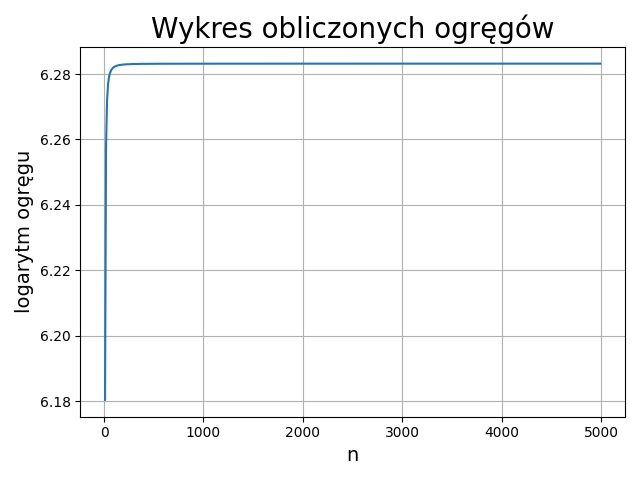
\includegraphics[width=\linewidth]{images/h1.png}
        \caption{Wartości obwodów $n$-kąta}
        \label{fig:h1}
    \end{minipage}\hfill
    \begin{minipage}{.45\textwidth}
        \centering
        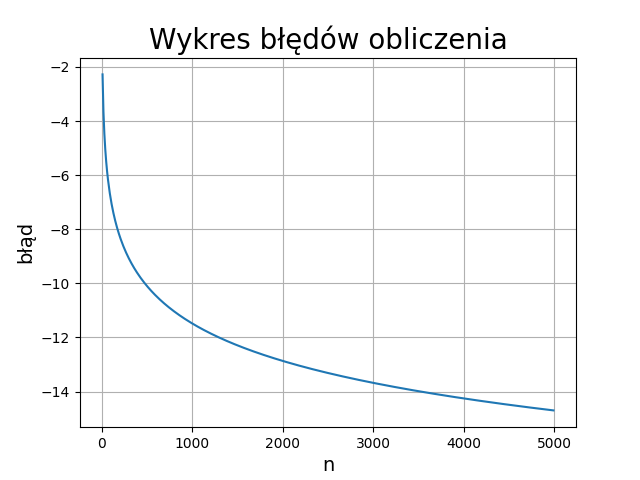
\includegraphics[width=\linewidth]{images/h1_blad.png}
        \caption{Wykres logarytmów błędów}
        \label{fig:h1_blad}
    \end{minipage}
\end{figure}

Z powyższych wykresów widać, że dla dużych wartości $n$ obwód wychodzi bliski $2\Pi$ a błędy są małe, co oznacza potwierdzenie powyższej hipotezy



\newpage

\section{Hipoteza 2: Suma wszystkich wektorów $w_{i}$ daje dokładnie wektor zerowy}

W celu sprawdzenia tej hipotezy obliczono sumy szystkich wektorów $w_{i}$ dla różnych wartości $n$ z przedziału $[10, 1000]$

Otrzymane wyniki umieszczono w tabeli \ref{tab:h2} oraz na rysunku \ref{fig:h2}

\begin{table}[htbp]
    \centering
    \begin{tabular}{| c | c | c |}
    \hline
    {$n$} & {$x$} & {$y$} \\
    \hline
    5 &  $0.00000000e+00$ & $-1.11022302 \times 10^{-16}$ \\
    10 & $3.05311332 \times 10^{-16}$ & $-4.44089210 \times 10^{-16}$ \\
    30 & $1.56819002 \times 10^{-15}$ & $-1.11022302 \times 10^{-15}$ \\
    50 & $2.55351296 \times 10^{-15}$ & $5.55111512 \times 10^{-16}$ \\
    70 & $2.96550978 \times 10^{-15}$ & $2.49800181 \times 10^{-16}$ \\
    90 & $-6.61450061 \times 10^{-15}$ & $7.35522754 \times 10^{-16}$ \\
    110 & $-4.72191730 \times 10^{-15}$ & $-5.27355937 \times 10^{-16}$ \\
    130 & $6.5683136 \times 10^{-15}$ & $-5.6898930 \times 10^{-16}$ \\
    150 & $3.73746173 \times 10^{-15}$ & $-1.07552856 \times 10^{-15}$ \\
    170 & $2.91943119 \times 10^{-15}$ & $-8.18789481 \times 10^{-16}$ \\
    190 & $5.96918348 \times 10^{-15}$ & $4.37150316 \times 10^{-16}$ \\
    200 & $7.71930263 \times 10^{-15}$ & $-2.08166817 \times 10^{-17}$ \\
    400 & $-2.70175050 \times 10^{-15}$ & $-6.59194921 \times 10^{-17}$ \\
    600 & $8.88657502 \times 10^{-15}$ & $-5.36029554 \times 10^{-16}$ \\
    800 & $-3.93870863 \times 10^{-14}$ & $-1.64972203 \times 10^{-15}$ \\
    1000 & $-1.79786097 \times 10^{-14}$ & $-7.99707522 \times 10^{-16}$ \\
    \hline
    \end{tabular}
    \caption{Sumy wektorów}
    \label{tab:h2}
\end{table}

\begin{figure}[!htb]
    \centering
        \centering
        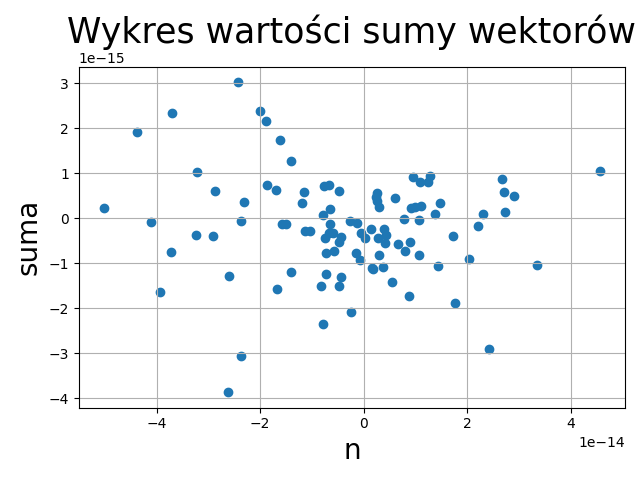
\includegraphics[width=10cm]{images/h2.png}
        \caption{Wykres sum wektorów}
        \label{fig:h2}
\end{figure}

Mimo że wartości są bliskie zeru, nie jest to dokładnie wektor zerowy o którym mowa w tej hipotezie. Wieć hipotezę 2 odrzucono

\newpage

\section{Hipoteza 3: Suma wektorów policzona innym sposobem}

Sumy współrzędnych wektorów $w_{i}$ policzono osobno: niech $X_{+}$ oznacza zbiór dodatnich współrzędnych $x$-owych wektorów $w_{i}$,a $X_{-}$ zbiór współrzędnych ujemnych; obliczono $S_{x+}$ sumując elementy zbioru $X_{+}$ w kolejności od najmniejszej do największej oraz $S_{x-}$ sumując elementy zbioru $X_{-}$ w kolejności od największej do najmniejszej; dodano do siebie $S_{x+}$ i $S_{x-}$.Dla współrzędnych $y$ zrobiono analogicznie


Wyniki obliczeń sum wektorów tym sposobem zamieszczono w tabeli \ref{tab:h3}




\begin{table}[htbp]
    \centering
    \begin{tabular}{| c | c | c |}
    \hline
    {$n$} & {$x$} & {$y$} \\
    \hline
    5 & $0.0$ & $0.0$ \\
    10 & $0.0$ & $-4.440892098500626 \times 10^{-16}$ \\
    20 & $-1.3322676295501878 \times 10^{-15}$ & $0.0$ \\
    30 & $1.3322676295501878 \times 10^{-15}$ & $-6.661338147750939 \times 10^{-16}$ \\
    40 & $2.6645352591003757 \times 10^{-15}$ & $0.0$ \\
    50 & $2.6645352591003757 \times 10^{-15}$ & $4.440892098500626 \times 10^{-16}$ \\
    60 & $-4.6629367034256575 \times 10^{-15}$ & $-4.440892098500626 \times 10^{-16}$ \\
    70 & $3.552713678800501 \times 10^{-15}$ & $2.220446049250313 \times 10^{-16}$ \\
    80 & $-6.661338147750939 \times 10^{-16}$ & $2.220446049250313 \times 10^{-16}$ \\
    90 & $-6.217248937900877 \times 10^{-15}$ & $4.440892098500626 \times 10^{-16}$ \\
    100 & $-6.661338147750939 \times 10^{-16}$ & $-8.881784197001252 \times 10^{-16}$ \\
    110 & $-4.6629367034256575 \times 10^{-15}$ & $-4.440892098500626 \times 10^{-16}$ \\
    120 & $-6.439293542825908 \times 10^{-15}$ & $-4.440892098500626 \times 10^{-16}$ \\
    130 & $5.773159728050814 \times 10^{-15}$ & $-8.881784197001252 \times 10^{-16}$ \\
    140 & $8.43769498715119 \times 10^{-15}$ & $-8.881784197001252 \times 10^{-16}$ \\
    150 & $3.552713678800501 \times 10^{-15}$ & $-1.1102230246251565 \times 10^{-15}$ \\
    160 & $-6.439293542825908 \times 10^{-15}$ & $0.0$ \\
    170 & $2.220446049250313 \times 10^{-15}$ & $-2.220446049250313 \times 10^{-16}$ \\
    180 & $3.1086244689504383 \times 10^{-15}$ & $-8.881784197001252 \times 10^{-16}$ \\
    190 & $7.105427357601002 \times 10^{-15}$ & $0.0$ \\
    200 & $7.105427357601002 \times 10^{-15}$ & $-4.440892098500626 \times 10^{-16}$ \\
    400 & $-3.774758283725532 \times 10^{-15}$ & $2.220446049250313 \times 10^{-16}$ \\
    600 & $1.021405182655144 \times 10^{-14}$ & $0.0$ \\
    800 & $-4.0190073491430667 \times 10^{-14}$ & $2.220446049250313 \times 10^{-16}$ \\
    1000 & $-1.7985612998927536 \times 10^{-14}$ & $-2.4424906541753444 \times 10^{-15}$ \\
    \hline
    \end{tabular}
    \caption{Wyniki sumy wektorów}
    \label{tab:h3}
\end{table}

Widać, że dla pewnych $n$ co najmniej jedna ze współrzędbych wynosi dokładnie $0.0$. A dla punktu $n = 5$ suma wynosi dokładnie wektor zerowy

Na rysunku \ref{fig:h3_} zamieszczono wyniki sum obliczonych w hipotezie 2 oraz w hipotezie 3.

Ponieważ dużo punktów się pokrywa, zrobiono nowe badanie. Wyliczono odległości każdego z wektorów od punktu $(0, 0)$, oraz wykonano odejmowanie od wartości sumy zwykłych wartości sumy wyliczonej powyższą metodą. Więc wartości nieujemne oznaczają, że dla pewnego $n$-kąta wyliczenie sumy wektorów powyższą metodą prowadzi do bardziej dokładnego wyniku. Wyniki zamieszczone na rysunku \ref{fig:h3}

Ponieważ nieujemnych wartości jest więcej, hipotezę, że przy takim sumowaniu wynik będzie bliższy wektorowi zerowemu potwierdzono
\begin{figure}[!htb]
    \centering
        \centering
        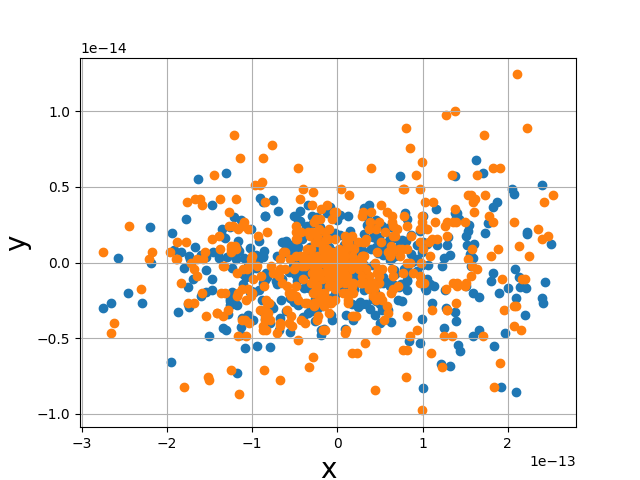
\includegraphics[width=10cm]{images/h3_.png}
        \caption{Wykres sum wektorów}
        \label{fig:h3_}
\end{figure}

\begin{figure}[!htb]
    \centering
        \centering
        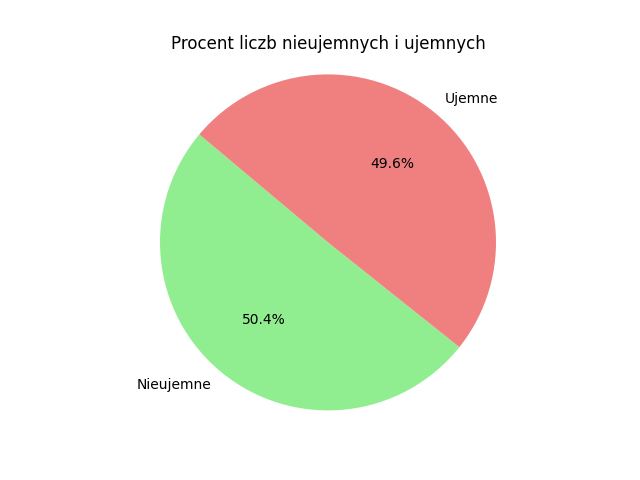
\includegraphics[width=10cm]{images/h3.png}
        \caption{Diagram badania odległości}
        \label{fig:h3}
\end{figure}

\newpage

\section{Hipoteza 4: Opisane zastosowanie metody Monte Carlo jest mniej efektywne niż metoda oparta o sumowanie wektorów}

W tabeli \ref{tab:h4} zamieszczono wyniki otrzymane w metodzie Monte Carlo. Jak widać z tych wyników obliczone wartości $\pi$ mają duży błąd, wykres błędów w zależności od liczby $n$ wylosowanych punktów można zobaczyć na rysunku \ref{fig:mc}

\begin{table}[htbp]
    \centering
    \begin{tabular}{| c | c | c |}
    \hline
    {$n$} & {$\pi$} & {błąd}  \\
    \hline
       100  & 3.04 & 0.10159265358979308 \\
       300  & 3.36 & 0.21840734641020676 \\
       500  & 3.216 & 0.07440734641020708 \\
       700  & 3.08 & 0.061592653589793045 \\
       900  & 3.2311111111111113 & 0.08951845752131815 \\
       1100 &  3.1745454545454543 & 0.03295280095566122 \\
       1300 &  3.129230769230769 & 0.012361884359024078 \\
       1500 &  3.144 & 0.002407346410207012 \\
       1700 &  3.1388235294117646 & 0.002769124178028548 \\
       1900 &  3.1242105263157893 & 0.01738212727400379 \\
    \hline
    \end{tabular}
    \caption{Wyniki otrzymane w metodzie Monte Carlo}
    \label{tab:h4}
\end{table}


\begin{figure}[!htb]
    \centering
        \centering
        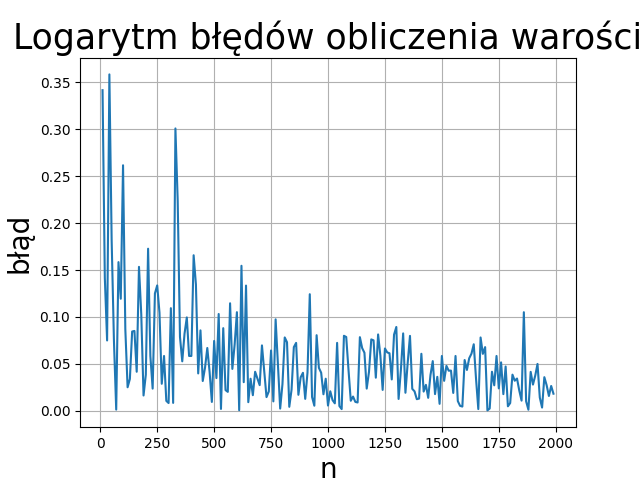
\includegraphics[width=10cm]{images/mc.png}
        \caption{Wykres błędu w metodzie Monte Carlo}
        \label{fig:mc}
\end{figure}

\newpage

\begin{figure}[!htb]
    \centering
        \centering
        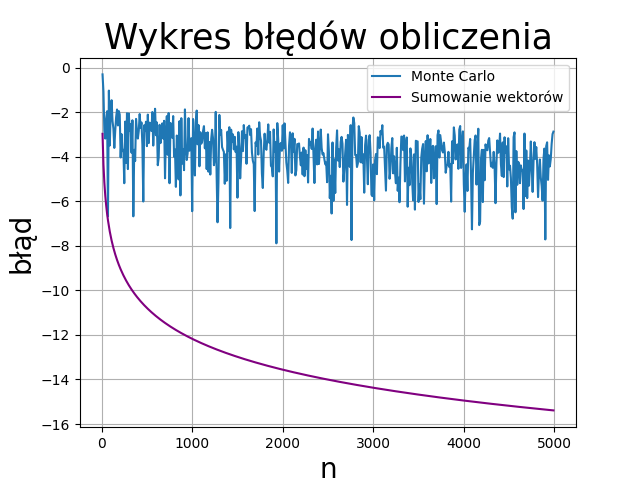
\includegraphics[width=10cm]{images/h4.png}
        \caption{Wykres błędu w metodzie Monte Carlo a przy sumowaniu wektorów}
        \label{fig:h4}
\end{figure}

Dla porównania efektywności obu metod (metody Monte Carlo a metody sumowania wektorów) zrobiono rysunek \ref{fig:h4}. Na tym rysunku widać, że błędy w metodzie Monte Carlo są znacznie większe niż przy sumowaniu wektorów. 

Obliczono błędy względne (średnie znaczenie): 
\begin{enumerate}
    \item Sumowanie wektorów: $0.0339\%$
    \item Monte Carlo: $5.472\%$
\end{enumerate}

Błąd względny metody Monte Carlo też jest znaczno większy niż błąd przy sumowaniu wektorów. Zatem hipotezę że zastosowanie metody Monte Carlo jest mniej efektywne niż metoda oparta o sumowanie wektorów potwierdzono

\newpage

\section{Hipoteza 5: Suma wektorów obliczona za pomocą kopca}

Została obliczona suma wektorów z użyciem kopca. Wyniki są przedstawione w tabeli \ref{tab:h5} oraz na rysunku \ref{fig:heap}


\begin{table}[htbp]
    \centering
    \begin{tabular}{ | c | c | c | }
      \hline
        {$n$} & {$x$} & {$y$} \\
        \hline
        5 & 0.0 & 0.0 \\
        10 & 0.0 & -2.220446049250313e-16 \\
        20 & -1.3322676295501878e-15 & 2.220446049250313e-16 \\
        30 & 1.3322676295501878e-15 & -4.440892098500626e-16 \\
        40 & 2.6645352591003757e-15 & 0.0 \\
        50 & 2.220446049250313e-15 & 2.220446049250313e-16 \\
        60 & -4.218847493575595e-15 & -6.661338147750939e-16 \\
        70 & 3.9968028886505635e-15 & 2.220446049250313e-16 \\
        80 & -1.1102230246251565e-15 & -2.220446049250313e-16 \\
        90 & -5.995204332975845e-15 & 2.220446049250313e-16 \\
        100 & -6.661338147750939e-16 & -4.440892098500626e-16 \\
        110 & -4.218847493575595e-15 & -8.881784197001252e-16 \\
        120 & -5.995204332975845e-15 & 4.440892098500626e-16 \\
        130 & 5.773159728050814e-15 & -4.440892098500626e-16 \\
        140 & 7.993605777301127e-15 & 0.0 \\
        150 & 4.440892098500626e-15 & -1.5543122344752192e-15 \\
        160 & -6.217248937900877e-15 & -2.220446049250313e-16 \\
        170 & 2.6645352591003757e-15 & 0.0 \\
        180 & 3.552713678800501e-15 & -1.3322676295501878e-15 \\
        190 & 7.105427357601002e-15 & 4.440892098500626e-16 \\
        200 & 7.105427357601002e-15 & -8.881784197001252e-16 \\
        400 & -4.440892098500626e-15 & -8.881784197001252e-16 \\
        600 & 7.993605777301127e-15 & -2.6645352591003757e-15 \\
        800 & -3.8413716652030416e-14 & -1.3322676295501878e-15 \\
        1000 & -1.7319479184152442e-14 & -4.440892098500626e-16 \\
       \hline
       \end{tabular}
       \caption{Wartości sumy wektorów przy sumowaniu za pomocą kopca}
       \label{tab:h5}
\end{table}

\begin{figure}[!htb]
    \centering
        \centering
        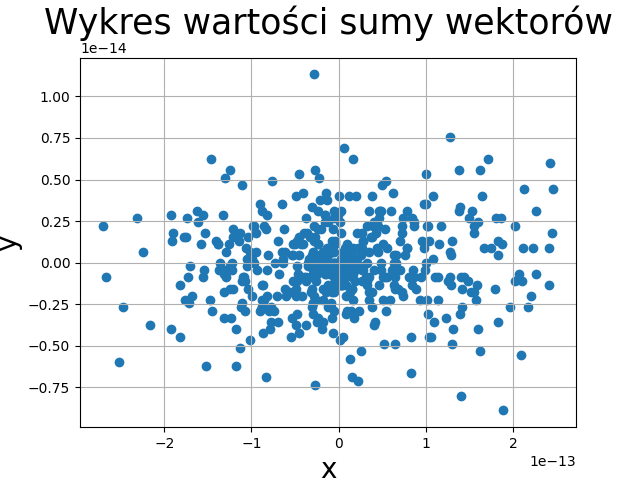
\includegraphics[width=10cm]{images/heap.png}
        \caption{Wykres wartości sum wektorów obliczonych za pomocą kopca}
        \label{fig:heap}
\end{figure}


Ponieważ wykres wektorów sum dla trzech metod sumowania nie będzie reprezentatywny, wykonano to samo badanie co w punkcie 3

\newpage
\begin{enumerate}
    \item Sumowanie kopcem a zwykłe sumowanie, rysunek \ref{fig:h2h5}

    Przeważają wartości nieujemne co oznacza, że sumowanie kopcem daje wynik bliższy zeru
    \item Sumowanie kopcem a sumowanie osobno wartości dodatnich i ujemnych, rysunek \ref{fig:h3h5}
    
    Przeważają wartości nieujemne, co oznacza, że sumowanie kopcem daje lepszy wynik 
    
\end{enumerate}

\begin{figure}[!htb]
    \centering
    \begin{minipage}{.45\textwidth}
        \centering
        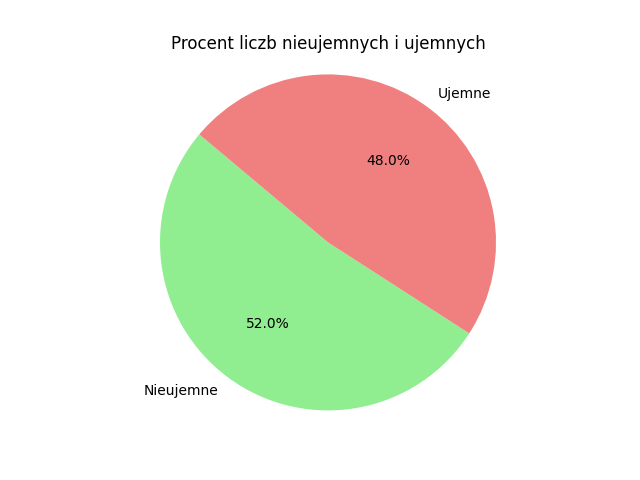
\includegraphics[width=\linewidth]{images/h2h5.png}
        \caption{Sumowanie kopcem a sumowanie zwykłe}
        \label{fig:h2h5}
    \end{minipage}\hfill
    \begin{minipage}{.45\textwidth}
        \centering
        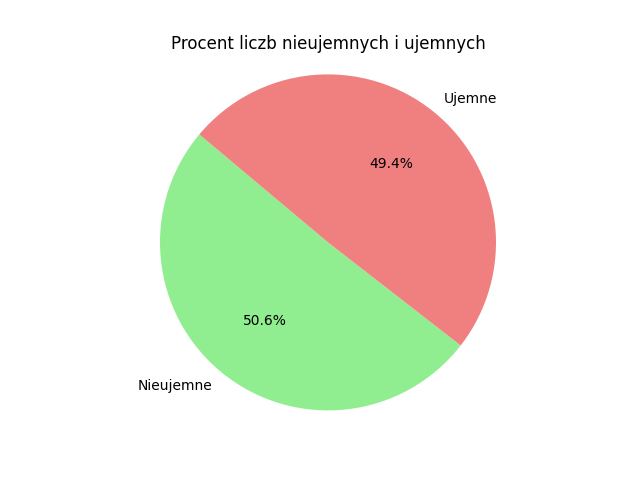
\includegraphics[width=\linewidth]{images/h3h5.png}
        \caption{Sumowanie kopcem a supowanie osobno}
        \label{fig:h3h5}
    \end{minipage}
\end{figure}

Podsumuwując sumowanie wektorów za pomocą kopca daje wynik bliższy wektorowi zerowemu, zatem hipotezę 5 potwierdzono

\newpage

\section{Podsumowanie}
Zostało wykonano obliczenie liczby $\Pi$ za pomocą dwóch metod. Sprawdzono, że zwiększając liczbę kątów wpisanego foremnego $n$-kąta można uzyskać obwód dowolnie bliski liczbie $2\Pi$. Badając efektywność wywnioskowano, że oblicznie za pomocą metody Monte Carlo jest mniej efektywne niż sumowanie długości wektorów. Również sprawdzając pewne hipotezy wywnioskowano, że sposób obliczania sumy wektorów na różne sposoby może prowadzić do uzyskania różnych wyników, najdokładniejszy wynik otrzymano przy wyliczaniu sumy za pomocą kopca

\end{document}